% 3. Protocol

\chapter{Methods and Materials}
\label{chap:methods}


\section{Setup for X-ray Absorption Measurement}
\label{sec:SetupAbsorb}

To measure the emission spectrum of the anode, a setup as shown in Fig. \ref{fig:setupabs} is used. The X-rays are generated in an X-ray tube (RR). A monochromator, realized in a rotatable single crystal (K), 
selects a specific wavelength of the X-ray spectrum depending on the angle 2$\theta$ set. After an aperture (B), the now nearly monochromatic X-ray radiation hits the sample holder (F). Into this holder the sample
can be inserted. After the radiation passed the sample holder, the intensity of the radiation is measured by a counting tube (Z) and the data is transferred to a computer. \cite{Anleitung}

\begin{center}
    \captionsetup{type = figure}
    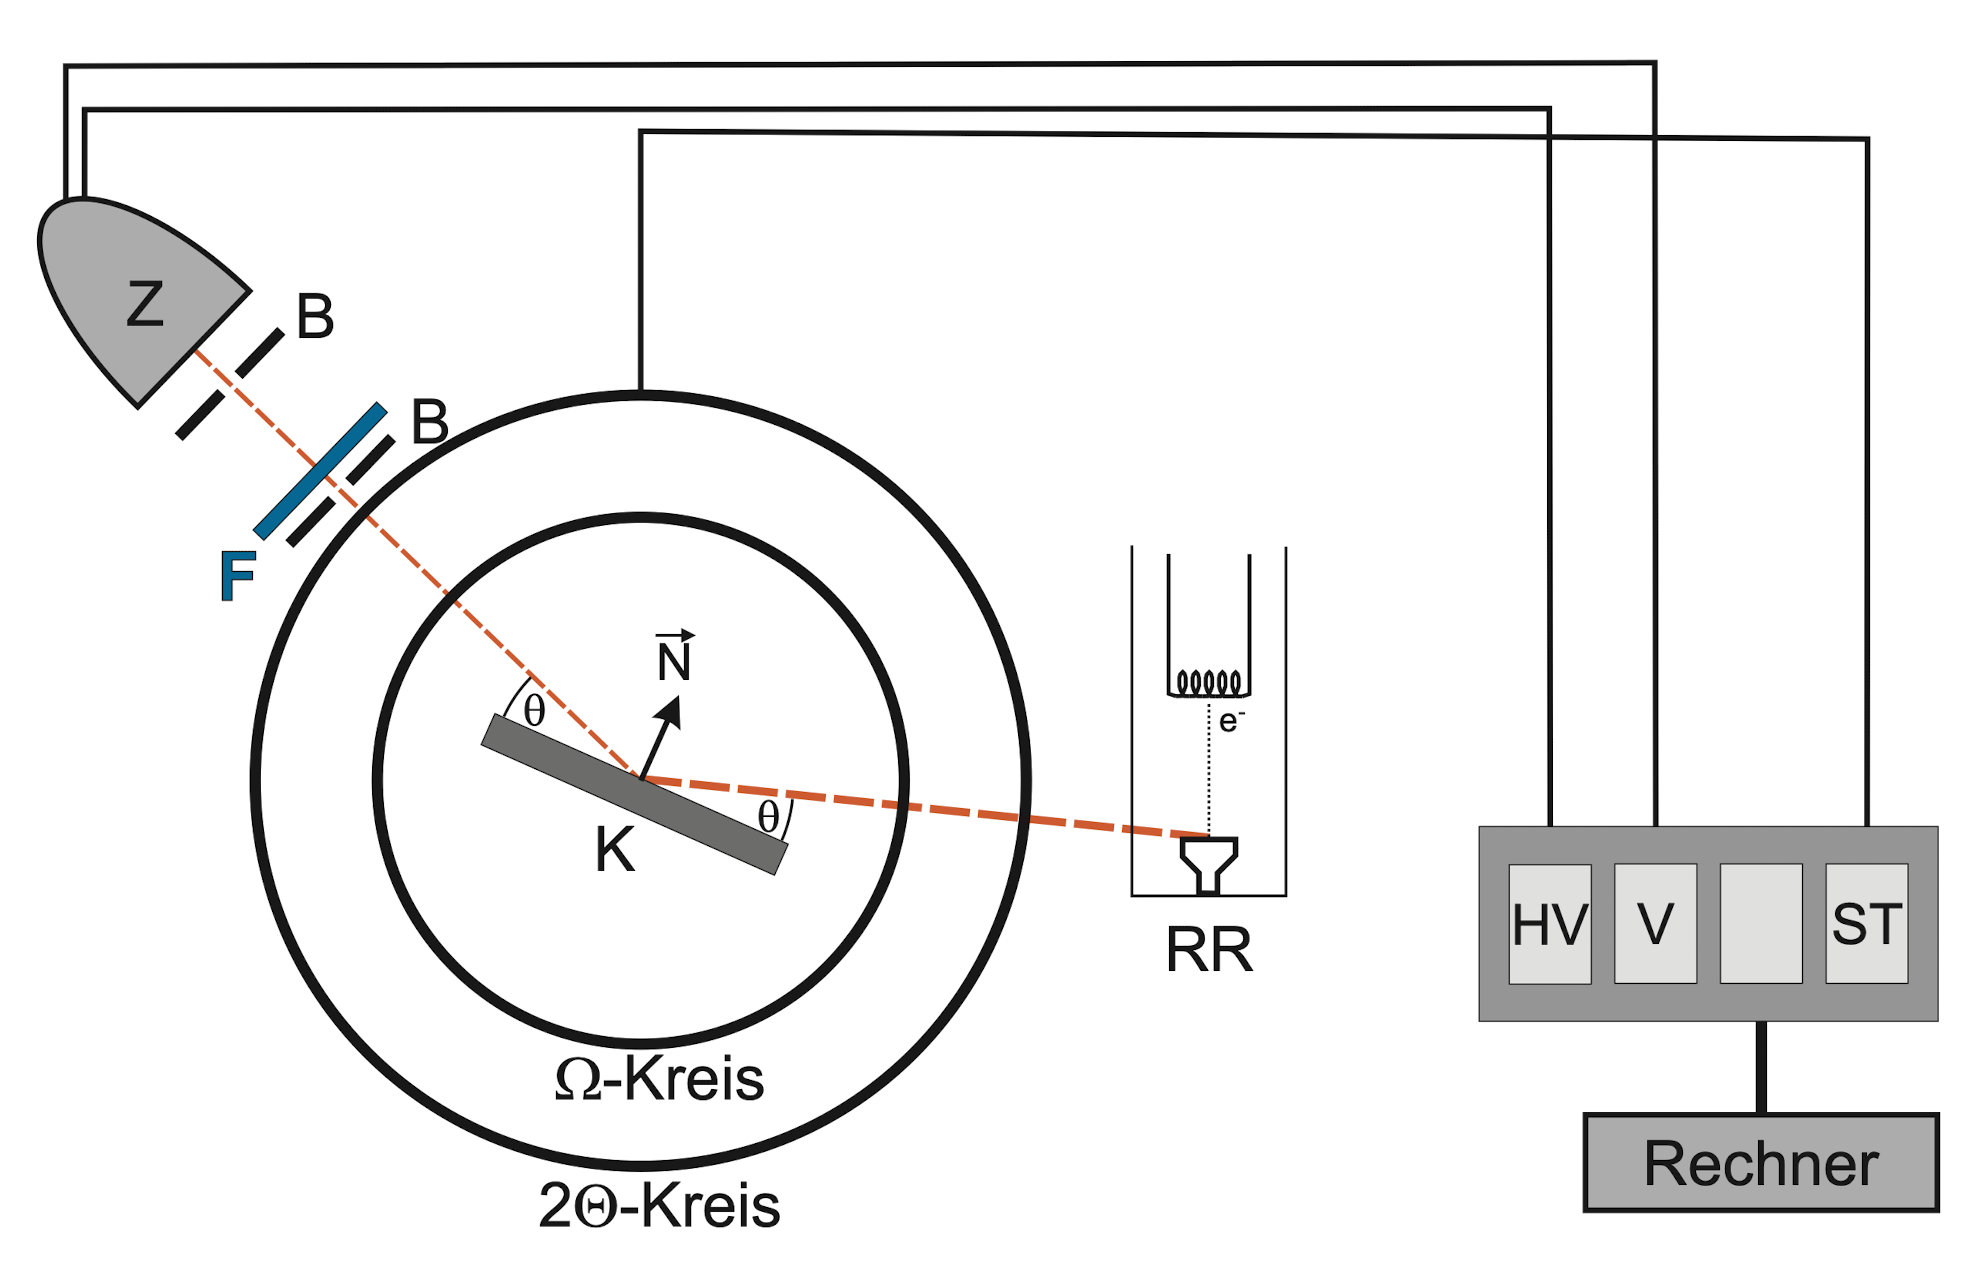
\includegraphics[width = 0.8\textwidth]{Pictures/SetupAbsorb.png}
    \captionof{figure}{
        Experimental setup of the absorption measurement. \cite{Anleitung}
    }
    \label{fig:setupabs}
\end{center}

\newpage
\section{Setup for Diffraction Measurement}
\label{sec:SetupDiff}

For the diffraction measurement we are using a similar setup to the setup used before. As depicted in Fig. \ref{fig:setupdiff}, the X-rays are generated in an X-ray tube (RR). Afterwards a monochromator selects one X-ray wavelength. 
The sample (S) is turned as the single crystal in the absorption setup. For each position the diffraction under 2$\theta$ is measured by a counting tube (Z) and the data is transferred to a computer.

\begin{center}
    \captionsetup{type = figure}
    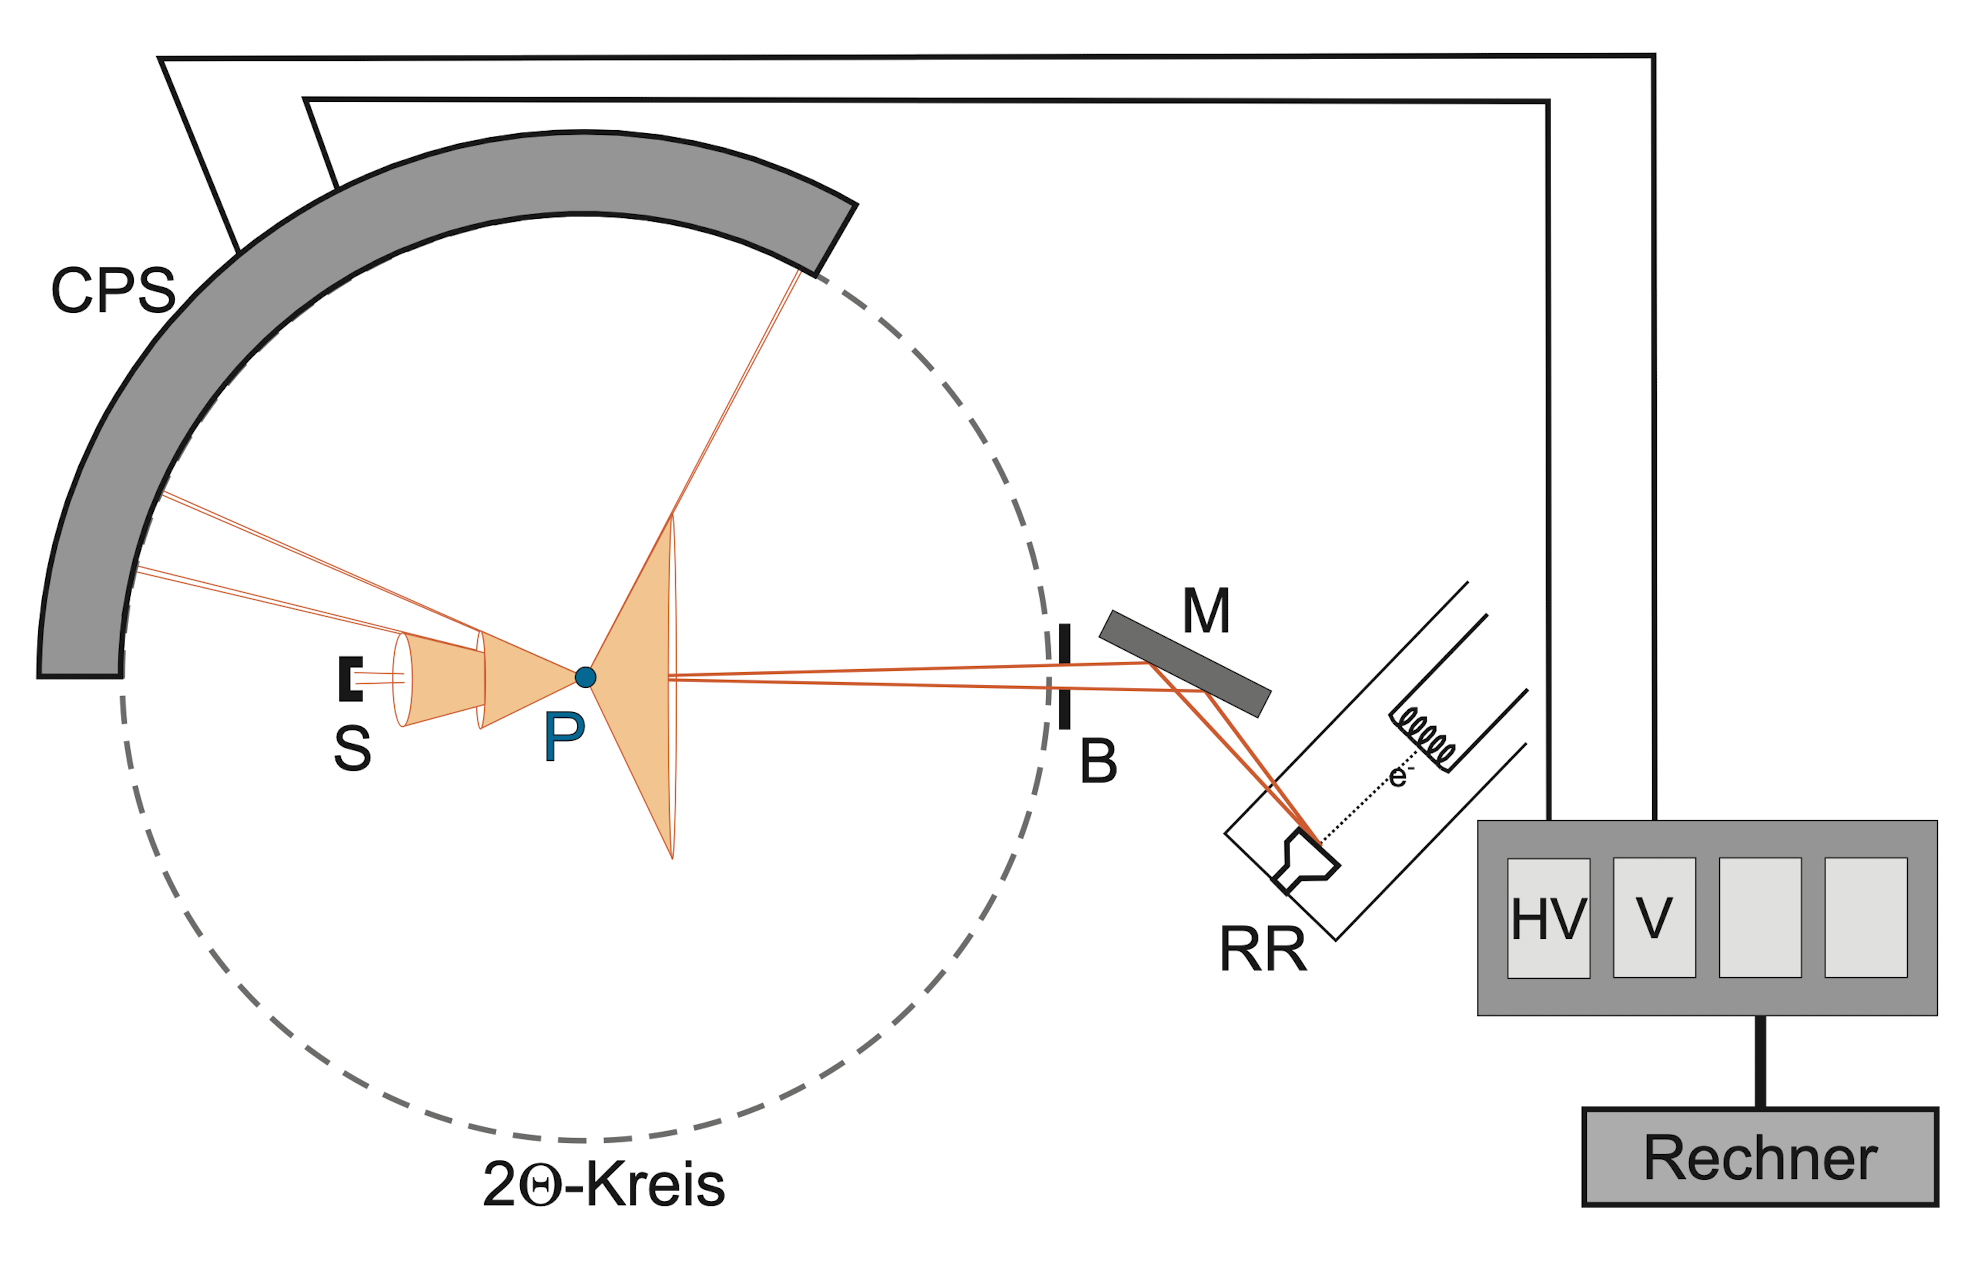
\includegraphics[width = 0.8\textwidth]{Pictures/SetupDiff.png}
    \captionof{figure}{
        Experimental setup of the diffraction measurement. \cite{Anleitung}
    }
    \label{fig:setupdiff}
\end{center}

In the sample preparation procedure, the crystal under examination (e.g., NaCl, glucose) is finely ground using a mortar. The resulting powder should possess a fine texture, barely detectable when rubbed between the fingers. Subsequently, the powder is carefully loaded into a sample holder, paying attention to a flat surface of the powder. Finally, the sample holder is inserted into the X-ray setup and the measurement is started. The measurement process runs for
approximately one week.  \cite{Anleitung}